\documentclass[a4paper,12pt,language=finnish,version=draft,hidechapters=true,includereferences=false,realtimesnewroman=false,sharelatex=false,emptyfirstpages=true]{utuftthesis}
\setcounter{secnumdepth}{2}
\setcounter{tocdepth}{2}

\addbibresource{Bibliografia.bib}
\begin{document}
\begin{comment}
Document template suitable for use as a LaTeX master-file for master's
thesis in University of Turku Department of Future Technologies.\\
\\
Compatible with: ShareLaTeX / PDFLaTeX / XeLaTeX.\\
\\
\\
{*}{*} HOW TO USE? {*}{*}\\
\\
Want to write a thesis? Clone this template in ShareLaTeX or fork
the department's thesis git project.\\
\\
The utuftthesis.cls defines a new thesis class, which is based on
the report class. It supports these new named parameters:

- paper: a4paper

- version: draft / final (default: draft) shows/hides {[}draft{]}
in the header

- language: finnish / english (default: finnish) affects the general
document appearance and hyphenation

- hidechapters: true / false (default: true) hides/shows the chapter/luku
text at the beginning of each Chapter

- includereferences: true / false (default: false) include reference
pages when calculating the total number of pages

- realtimesnewroman: true / false (default: false) use Times New Roman
instead of LaTeX fonts with XeLaTeX. Requires the font to be installed
on the system / provided in the document directory. Other fonts can
be defined with \textbackslash setmainfont.

- sharelatex: true / false (default: false) don't attempt to use (c)
system fonts, instead read them from the project repository

- emptyfirstpages: true / false (default: true) clear the headers/footers
for the 1st pages of text chapters

Traditionally the best places to learn (La)TeX are probably the manual
pages for each package http://www.ctan.org/ and http://www.ctan.org/tex-archive/info/lshort/english/lshort.pdf.
This new version (2.0) should be compatible with xelatex and biblatex
which means that all source files can freely use normal UTF-8 text
without resorting to \textquotedbl\textquotedbl legacy hacks\textquotedbl .\\
\\
Note that PDF/A requirements don't allow PDF links, but if you want
to provide a user friendly version of the thesis with links, use \textbackslash hyperref\\
\\
\\
{*}{*} Maintenance {*}{*}\\
\\
Workflow: https://gitlab.utu.fi/ttweb/thesis -> master .lyx document
exported as .tex documents -> repository content dumped to the sharelatex
project template

Want to fix something in the template? Send a merge.\\
\\
Relies on utuftthesis.cls for the document class definitions.
\end{comment}


\pubyear{2019}
\pubmonth{11}

\pubtype{luk}
\title{Funktionaalisen- ja olioparadigman suorituskykyvertailu Scala-kielellä}
\author{Jaakko Paju}

\maketitle
%
\keywords{suorituskyky, funktionaalinen ohjelmointi, ohjelmointiparadigma, Scala}

\begin{abstract}
Funktionaalisesta ohjelmoinnista lainattuja ominaisuuksia lisätään jatkuvasti perinteisiin imperatiivisiin ohjelmointikieliin. Yksi funktionaalisen ohjelmoinnin keskeisimmistä käsitteistä on muuttumattomat arvot. Muuttumattomien arvojen ja tietorakenteiden käyttö saattaa lisätä kopioimisen tarvetta ja samalla heikentää ohjelman suorituskykyä.

Tutkielman tarkoituksena on perehtyä funktionaalisten ohjelmien suorituskykyyn vaikuttaviin seikkoihin sekä verrata funktionaalisen paradigman suorituskykyä imperatiiviseen paradigmaan. Vertailut tehdään Scala-kielellä, sillä se tukee kumpaakin edellä mainittua paradigmaa. Tutkielmassa keskitytään järjestettyjen muuttumattomien ja muuttuvien kokoelmien suorituskyvyn vertailuun. Suorituskykyä tutkitaan useamman eri mittauksen pohjalta, ja mittauksien tuloksia vertaillaan toisiinsa.

Mittauksissa ei havaittu säännönmukaisia eroja muuttumattomien ja muuttuvien kokoelmien suorituskyvyssä, vaikka muuttuvat kokoelmat olivat joissain mittauksissa hieman muuttumattomia suorituskykyisempiä. Suurin vaikutus suorituskykyyn on tarkoituksenmukaisen tietorakenteen valitsemisella riippumatta onko kyseessä muuttuva vai muuttumaton kokoelma.

Tutkielman pohjalta ei voida tehdä johtopäätöksiä funktionaalisen paradigman kokonaisvaltaisesta vaikutuksesta ohjelman suorituskykyyn. Kokonaisvaltaisten vaikutusten arvioimiseksi tulisi tutkia myös muita funktionaalisen paradigman keskeisiä käsitteitä, kuten sulkeumia, hahmontunnistusta ja rekursiota.
\end{abstract}


% empty pagestyle for table of contents etc.
% otherwise you'll get simple page style with roman page numbers
\pagestyle{empty}

% mandatory
\tableofcontents

% if you want a list of figures
%\listoffigures

% if you want a list of tables
%\listoftables

% 'list of acronyms'
%   - you may not need this at all
%   - create a chapter called List Of Acronyms (or whatever), which
%     should contain all your acronym definitions, e.g. 
%     \chapter{List Of Acronyms} 
%   - the secnumdepth trickery is needed because acronyms are as a
%     standard chapter and we are faking '\listofacronyms'
%
%\setcounter{secnumdepth}{-1}
%\input{your acronym chapter's file name}
%\setcounter{secnumdepth}{2}% setup page numbering, page counter, etc.%
\begin{comment}
The thesis starts here.

To better organize things, create a new tex file for each chapter
and input it below.

Avoid using the å, ä, ö or <space> characters in referred names and
underscores \_ in file names (may break hyperref).

Good luck!
\end{comment}

\chapter{Johdanto} \label{Johdanto}
Funktionaalinen ohjelmointi kasvattaa suosiotaan jatkuvasti. Useisiin yleiskäyttöisiin ja alunperin imperatiivisiin ohjelmointikieliin on lisätty ominaisuuksia funktionaalisesta ohjelmoinnista. Esimerkiksi suositut oliokielet Java, Python ja C++ ovat kaikki lainanneet funktionaalisesta ohjelmoinnista anonyymit sekä korkeamman asteen funktiot.

Funktionaalisen paradigman keskeisistä käsitteitä ovat muuttumattomat arvot ja tietorakenteet. Muuttumattomien arvojen käyttäminen usein lisää kopioimisen tarvetta verrattuna ohjelmiin, joissa käytetään muuttuvia arvoja. Kopioimisen seurauksena muistia pitää varata ja vapauttaa useammin kuin muuttuvia arvoja käytettäessä. Tämä herättää kysymyksen funktionaalisten ohjelmien suorituskyvystä verrattuna imperatiivisiin ohjelmiin.

Tutkielmassa perehdytään tarkastelemaan millaisia vaikutuksia funktionaalisella paradigmalla on suorituskykyyn verrattuna olioparadigmaan. Tutkielman suorituskykyvertailut keskittyvät Scala-ohjelmointikieleen, sillä se on suunniteltu tukemaan sekä funktionaalista että olioparadigmaa, jolloin suorituskyvyn vertailu näiden kahden paradigman välillä on mielekästä ja suoraviivaista. Tarkastelu kohdistuu erityisesti muuttumattomiin kokoelmiin. \todo{Lisää toinen tutkittava aihe} Tutkielma on suoritettu perehtymällä aihetta käsittelevään kirjallisuuteen.

Luvussa \ref{Ohjelmointiparadigmat} esitellään molemmat vertailun kohteena olevat paradigmat. Luvussa \ref{Scala} esitellään Scala-kielen rakenteet, ja miten ne tukevat kumpaakin paradigmaa. Luvussa \ref{Kokoelmat} tarkastellaan Scalan standardikirjaston muuttumattomien kokoelmien suorituskykyä ja verrataan sitä muuttuvien kokoelmien suorituskykyyn. \todo{Varmista että suorituskykyä oikeasti verrataan muuttuviin kokoelmiiin} Viimeisenä luvussa \ref{Yhteenveto} esitellään johtopäätökset ja kootaan tutkielman tulokset.

\todo{Lisää esittely toisesta tutkittavasta aiheesta}

\chapter{Scala} \label{Scala}
Scala on staattisesti tyypitetty moniparadigmainen käännettävä ohjelmointikieli, joka yhdistää funktionaalisen ohjelmoinnin ja olio-ohjelmoinnin ominaisuuksia. Scala on korkean tason kieli ja sen syntaksi on kompaktia ja eleganttia. Scalan kääntäjä ja tyyppijärjestelmä takaavata tyyppiturvallisuuden kääntämisen aikana muutamaa poikkeusta lukuunottamatta. Scala-koodi on tarkoitettu käännettäväksi Javan tavukoodiksi, ja se mahdollistaa Java-kirjastojen käyttämisen suoraan Scalasta. Tavukoodia ajetaan Javan virtuaalikoneessa (JVM). Tässä tutkielmassa tarkastellaan Scalan versiota 2.12.10.
\cite[Introduction]{tourOfScala}
\cite[Luku 2]{prorgrammingInScala3rd}


\section{Muuttujat} \label{Muuttujat}
Scalassa on tavallisten muuttujien lisäksi vakioita, jotka ovat muuttujia, joiden arvoa ei alustuksen jälkeen voi muuttaa. Vakion määrittelyyn käytetään avainsanaa \code{val} ja muuttujan määrittelyyn \code{var}. Funktionaalisessa Scalassa käytetään pääasiassa \code{val}-avainsanalla määriteltyjä muuttujia, ja imperatiivisessa tyylissä voidaan käyttää molempia.

Muuttujan nimen jälkeen määritellään muuttujan tyyppi, joka erotetaan muuttujan nimesta kaksoispisteellä. Esimerkiksi \code{val x: Int = 1} alustaa kokonaislukuvakion x, jonka arvo on 1. Muuttujan tyyppimäärittelyn voi jättää myös kirjoittamatta, sillä Scala-kääntäjä osaa yleensä päätellä muuttujan tyypin asetetun arvon perusteella. Edellisen esimerkin voi siis halutessaan kirjoittaa muodossa \code{val x = 1}, ja Scala osaa päätellä muuttujan olevan tyypiltään kokonaisluku.
\cite[Basics]{tourOfScala}

Muuttujat ovat myös staattisesti tyypitettyjä, joten muuttujan tyyppi ei voi muuttua ajon aikana. Scalassa myös funktiot ovat arvoja, joten niitä voidaan sijoittaa muuttujiin. Esimerkiksi \code{val add1 = (x: Int) => x + 1} luo \textit{funktioliteraalin} ja sijoittaa sen muuttujaan nimeltä add1. Funktioita käsitellään tarkemmin luvussa \ref{MetoditJaFunktiot}.
\cite[Luku 1]{prorgrammingInScala3rd}


\section{Tietotyypit}
Scala on puhtaasti oliokieli, eli kaikki arvot ja muuttujat ovat olioita. Jokainen Scalan tietotyyppi perii luokan \code{Any} ja luokka \code{Nothing} on jokaisen tietotyypin alaluokka. Scalassa luokka voi olla arvoluokka tai viiteluokka. Arvoluokat perivät luokan \code{AnyVal} ja niihin ei voi sijoittaa null-arvoa. Viiteluokat perivät luokan \code{AnyRef}, joka on tyyppialias Javan luokalle \code{Object}. Jokaisen viiteluokan alaluokka on \code{Null}. Tietotyyppien hierarkia on kuvattu kuvassa \ref{tyyppihierarkia}.
\cite[Luku 5]{prorgrammingInScala3rd}

\begin{figure}[h]
    \centering 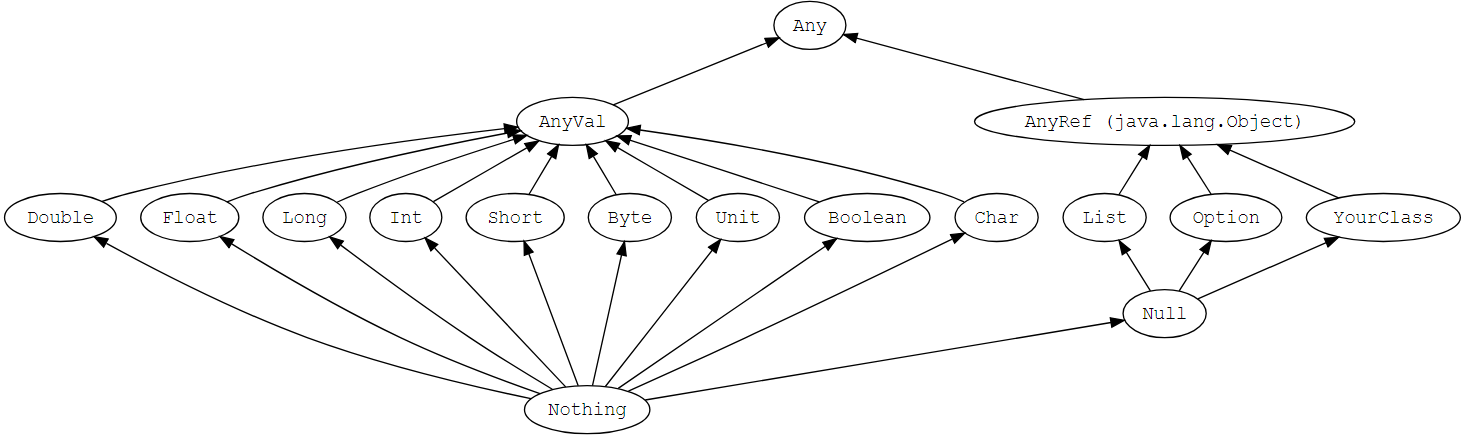
\includegraphics[width=1\textwidth]{kuvat/typehierarchy}
    \caption{Scalan luokkahierarkia}
    \label{tyyppihierarkia}
\end{figure}

Alkeistietotyyppejä kuvaavat arvoluokat \code{Byte}, \code{Short}, \code{Int}, \code{Long}, \code{Char}, \code{Float}, \code{Double}, \code{Boolean} ja \code{Unit}. Kaikki paitsi \code{Unit} vastaavat Javan vastaavia kääreluokkia. \code{Unit} on erityinen tietotyyppi, joka kuvastaa funktion tyhjää paluuarvoa. Sen voi ajatella vastaavan Javan void-avainsanaa. Merkkijonoja Scalassa kuvaa tietotyyppi \code{String}, joka on tyyppialias Javan merkkijonoa kuvaavalle tietotyypille.
\cite[Luku 5]{prorgrammingInScala3rd}

Scalan alkeistietotyypit muutetaan käännösvaiheessa primitiivityypeiksi, esimerkiksi Scalan \code{Int} käännetään 32-bittiseksi sanaksi, aivan kuten Javan \code{int}. Tämä takaa yhteensopivuuden Java-kirjastojen kanssa. Se parantaa myös suorituskykyä, sillä primitiiviarvolle ei tarvitse allokoida muistia ajon aikana.
\cite[Luku 6]{prorgrammingInScala3rd}


\section{Kontrollirakenteet}

\subsection{Ehtolauseet}
Ehtolauseita kirjoitetaan Scalassa \textit{if/else}-lausekkeiden avulla. Lauseketta voi käyttää imperatiiviseen tyyliin eli jos ehto arvioituu todeksi, suoritetaan if-lohko, muuten else-lohko.
\begin{lstlisting}
    val x = true
    if (x) {
        println("True")
    } else {
        println("False")
    }
    // Tulostaa "True"
\end{lstlisting}
Scalan if-lausekkeella on myös arvo, eli if-lauseke palauttaa arvon. Arvon palauttava if-lauseke on siis funktionaalinen, koska sillä on arvo. Esimerkiksi \codebl{val y = if (x >= 0) \"positive\" else \"negative\"} asettaa muuttujan \code{y} arvoksi joko merkkijonon "positive" tai "negative", riippuen muuttujan \code{x} arvosta. Huomattavaa on myös, että if-lauseke voidaan kirjoittaa yhdelle riville ilman aaltosulkeita. 
\cite[Luku 2.1]{scalaForTheImpatient}
        
\subsection{Silmukat}
Silmukoita Scalassa on kolmenlaisia: \code{while}, \code{do} ja \code{for}. While-silmukka suorittaa sitä seuraavaa lohkoa 0-n kertaa, kunnes annettu ehto arvioituu epätodeksi. Do-silmukka toimii vastaavalla tavalla, mutta sitä suoritetaan 1-n kertaa.
\begin{lstlisting}
    val x = false
		while (x)
			println("while")
		
		do
			println("do")
        while (x)
\end{lstlisting}
Yllä oleva esimerkki ei suorita while-silmukkaa kertaakaan, ja do-silmukan kerran.
\cite[Luku 2.5]{scalaForTheImpatient}

Scalan \code{for}-lauseke on monipuolisempi kuin monissa muissa kielissä. Sitä voi käyttää perinteiseen tapaan silmukkana, jolloin for-lausekkeen \textit{generaattori} antaa määriteltyjä arvoja yksi kerrallaan muuttujan \code{i} kautta. Lauseketta voidaan käyttää myös usean generaattorin kanssa ja arvoja voidaan suodattaa lausekkeen sisällä. Kuten if-lauseke, myös for-lauseke voi palauttaa arvon. Seuraavaksi esimerkki kummastakin käyttötavasta.
\begin{lstlisting}
    for (i <- 1 to 10)
        println(i)
\end{lstlisting}
Silmukkana lauseketta voi käyttää yllä olevan esimerkin tapaan tulostamaan kaikki numerot yhdestä kymmeneen.
\begin{lstlisting}
    val res = for {
        x <- 1 to 10
        if x % 2 == 0
    } yield (x * 2) // Vector(4, 8, 12, 16, 20)
\end{lstlisting}
Yllä olevassa esimerkissä luodaan kokonaisnumerovektori yhdestä kymmeneen, suodatetaan parilliset arvot, palautetaan jäljelle jäääneet arvot kahdella kerrottuna ja asetetaan palautettu vektori muuttujaan \code{res}. Tälläinen \code{for}-lauseke on yleinen funktionaalisessa Scalassa.
\cite[Luku 2.6]{scalaForTheImpatient}


\section{Metodit ja funktiot} \label{MetoditJaFunktiot}
Jokainen operaatio Scalassa on metodikutsu. Myös tavanomaiset aritmeettiset operaattorit on toteutettu metodikutsuina. Esimerkiksi kahden kokonaisluvun yhteenlasku \code{1 + 2} on lyhyempi versio metodikutsusta \code{1.+(2)}. Scalassa on mahdollista määritellä funktio kahdella tavalla: olion metodiksi tai funktioliteraaliksi. Metodi voidaan määritellä \code{def}-avainsanalla.
Scalassa funktio palauttaa automaattisesti viimeisen lausekkeensa arvon, joten \code{return}-avainsanan käyttö on vapaaehtoista ja sitä käytetään vain harvoin.
\cite[Luku 1.4]{scalaForTheImpatient}
\cite[Basics]{tourOfScala}

\subsection{Funktioliteraalit}
Funktioliteraali on funktio, jota käsitellään kuten mitä tahansa muuttujaa. Yleensä funktioliteraali sijoitetaan muuttujaan tai annetaan parametriksi toiselle funktiolle. Kuten muillakin muuttujilla, funktioilla ja metodeilla on Scalassa aina tyyppi. Tyypin voi määritellä eksplisiittisesti, mutta monesti Scala osaa päätellä funktion tyypin.
Seuraavassa esimerkissä määritellään kummallakin tavoilla funktio, joka kertoo onko parametrina annettu kokonaisluku parillinen. Funktion tyyppi on siis \code{Int => Boolean}.
\cite[Luku 8]{prorgrammingInScala3rd}
\begin{lstlisting}
    def isEven1(x: Int): Boolean = x % 2 == 0
    val isEven2: (Int => Boolean) = x => x % 2 == 0
\end{lstlisting}

\subsection{Korkeamman asteen funktiot}
Funktio voi ottaa parametriksi toisen funktion tai palauttaa funktion. Tälläisiä funktioita kutsutaan \textit{korkeamman asteen funktioiksi}. Korkeamman asteen funktiot ovat yksi funktionaalisen ohjelmoinnin kulmakivistä. Seuraavassa esitellään korkeamman asteen funktio, joka ottaa parametrina kokonaisluvun sekä funktion kokonaisluvusta kokonaislukuu, ja palauttaa kutsuu tätä funktiota parametrin kokonaisluvulle.
\begin{lstlisting}
    def mapValue(v: Int, m: Int => Int): Int = m(v)
    
    def double(x: Int): Int = x * 2
    
    mapValue(2, double)
    mapValue(2, _ * 3)
\end{lstlisting}
Kuten yllä olevasta esimerkistä huomataan, annetaan \code{double}-funktio parametrinä ihan kuten mikä tahansa muukin muuttuja. Esimerkin viimeisellä rivillä käytetään funktioliteraalia \code{_ * 3}, joka on lyhyempi muoto funktioliteraalille \code{x => x * 3}.
\cite[Luku 12]{scalaForTheImpatient}


\section{Luokat ja oliot} \label{LuokatJaOliot}
Scalassa on useita erilaisia luokka- ja oliotyyppejä sekä tapoja luoda instansseja luokista. Tässä luvussa esitellään pääpiirteittäin erilaiset luokkatyypit.

\subsection{Class} \label{class}
Luokka voidaan määritellä Scalassa \code{class}-avainsanalla. Luokka voi olla tyhjä tai se voi sisältää metodeita ja muuttujia. Luokasta luodaan instanssi \code{new}-avainsanalla. Luokan sisältämät kentät voidaan määritellä konstruktorissa heti luokan nimen jälkeen suluissa. Konstruktorissa määritellyt kentät ovat oletuksena \code{private val}. Luokasta saadaan uusi instanssi \code{new}-avainsanan avulla. Ihmistä kuvaava luokka ja instanssi voidaan määritellä seuraavalla tavalla:
\begin{lstlisting}
    class Person(val name: String, var age: Int) {
        def isAdult = age >= 18
    }
    val p = new Person("Matti", 30)
\end{lstlisting}
Luokassa Person on kaksi kenttää: julkinen muuttumaton kenttä nimi ja julkinen muutettava ikä. Lisäksi luokassa on metodi, joka kertoo onko henkilö täysi-ikäinen.
\cite[Classes]{tourOfScala}


\subsection{Case class} \label{caseclass}
Scalassa on myös erityisiä case-luokkia, joita käytetään yleensä kuvaamaan muuttumatonta dataa. Case-luokka määritellään kuten tavallinen luokka, mutta konstruktorissa määriteltävät kentät ovat oletuksena \code{public val}. Case-luokkaan voidaan määräitellä metodeita samoin kuin tavalliseenkin luokkaan. Case-luokan instanssia luotaessa ei tarvitse käyttää \code{new}-avainsanaa. Puhelinmallia kuvaava case-luokka ja instanssi voidaan määritellä seuraavalla tavalla:
\begin{lstlisting}
    case class Phone(brand: String, model: String)
    val p = Phone("Google", "Pixel4")
\end{lstlisting}
Scala-kääntäjä lisää case-luokkiin \code{toString}-, \code{hashCode}-, \code{equals}- ja \code{copy}-metodeita oletustoteutuksilla. Lisäksi kääntäjä lisää \textit{kumppaniolioon} \code{apply}-tehdasmetodin, jonka avulla uusien instanssien luonti tapahtuu.
\cite[Luku 15]{prorgrammingInScala3rd}

Tavallisia luokkia käytetään varsinkin oliotyylisessä ohjelmoinnissa, kun taas case-luokat ovat käytössä erityisesti funktionaalisessa Scalassa, kun halutaan käyttää muuttumattomia olioita. Tavallisten luokkien ja case-luokkien yhtäsuuruusvertailut eroavat toisistaan merkittävästi. Tavallisia luokkia verrataan viittauksen mukaan, eli osoittaako viittaus samaan olioon JVM:ssä. Case-luokkien yhtäsuuruutta verrataan olion kenttien arvon mukaan.
\cite[Luku 15]{prorgrammingInScala3rd}

\subsection{Singleton-oliot} \label{singleton-oliot}
Useat muut oliokielet tarjoavat mahdollisuuden kirjoittaa staattisia luokkia tai staattisia kenttiä luokkiin. Scalassa tälläistä staattisuutta ei ole, vaan vastaava toiminnallisuus mahdollistetaan erityisien \textit{singleton}-olioiden kautta. Singleton-oliosta on ajon aikana olemassa vain yksi instanssi, ja Scala luo sen automaattisesti. Singleton-olion on mahdollista periä luokka. Viittaaminen olioon tapahtuu yksinkertaisesti olion nimellä.
\cite[Singleton objects]{tourOfScala}

Singleton-oliota voidaan kutsua myös kumppaniolioksi, jos se on määritelty saman nimisen luokan yhteydessä. Kumppanioliot näkevät ilmentymiensä yksityiset kentät, ja ilmentymät näkevät kumppaniolionsa yksityiset kentät. Luvun \ref{caseclass} Phone-luokalle voidaan luoda kumppaniolio seuraavalla tavalla:
\begin{lstlisting}
    object Phone {
        def iphone11 = new Phone("Apple", "iPhone 11")
    }
    val iphone = Phone.iphone11
\end{lstlisting}
Tässä tapauksessa kumppanioliossa on vain yksi metodi, jonka avulla voidaan luoda helposti instansseja.
\cite[Luku 4]{prorgrammingInScala3rd}


\subsection{Piirretyypit} \label{piirretyypit}
Piirretyyppejä käytetään Scalassa määrittelemään olioiden tarjoamien palveluiden rajapintoja ja mahdollistamaan ohjelmakoodin uudelleenkäytettävyyttä. Uusi piirretyyppi luodaan \code{trait}-avainsanalla. Piirretyyppien on myös sallittua periä toisia piirretyyppejä tai luokkia. Myös singleton-olioihin on mahdollista liittää piirretyyppejä. Piirretyypin voi ajatella olevan Javan rajapintaluokan ja abstraktin luokan yhdistelmä.
\cite[Luku 6 ja 12]{prorgrammingInScala3rd}

Piirretyypin jäseniksi voidaan määritellä metodeita tai muuttujia. Jäsenet voivat olla abstrakteja tai konkreetteja. Abstraktille jäsenelle tulee toteuttavan luokan tarjota toteutus, kun taas konkreettielle jäsenille ei. Yhdessä piirreluokassa voi olla sekä abstrakteja että konkreetteja jäseniä. Tietyissä erityistapauksissa metodi voidaan merkitä abstraktiksi, vaikka sille on annettu toteutus piirretyypissä.
\cite[Luku 10]{scalaForTheImpatient}


\printbibliography

\begin{comment}
Create your appendix chapters with command \textbackslash appchapter\{some
name\} instead of \textbackslash chapter\{some name\} for the automagic
page counting to work!
\end{comment}

\end{document}
